\begin{enumerate}[label=\thesubsection.\arabic*.,ref=\thesubsection.\theenumi]
\numberwithin{equation}{enumi}
\item
For the Wein-bridge oscillator of Fig \ref{fig:ee18btech11044_3_tikz_1}, use the expression for loop gain in Eq \ref{eq:ee18btech11044_3_1}  to find the poles of the closed-loop system. Give the expression for the pole , Q and use it to show that to locate the poles in the right half of s plane, $\frac{R_2}{R_1}$ must be selected to be greater than 2. 

\begin{figure}[!hbt]
	\begin{center}
			\resizebox{\columnwidth}{!}{\begin{circuitikz}
\ctikzset{bipoles/length=1cm}

\draw 
(0, 0) node[op amp] (opamp) {}
(opamp.-) -- (-1,0.35) -- (-1.5,0.35) to[R=$R_1$] (-3,0.35) -- (-3,0.33)node[ground]{}
(-1,0.35)-- (-1,1) to[R=$R_2$] (2,1) -- (2,0){}
(opamp.out)--(2,0){}
(opamp.+) -- (-1,-0.35) -- (-1,-1.5) to[C=$C$] (0.5,-1.5) to[R=$R$] (2,-1.5) -- (2,0){}
(-1,-1.5) -- (-1,-1.75)to[R=$R$] (-1,-2.5) -- (-1,-2.57)node[ground]{}
(0.5,-1.5) -- (0.5,-1.75) to[C=$C$] (0.5,-2.5) -- (0.5,-2.57)node[ground]{}
node at (2.3,0){$V_{out}$}



;\end{circuitikz}
}
	\end{center}
\caption{}
\label{fig:ee18btech11044_3_tikz_1}
\end{figure}


\item Compare the basic structure for a sinusoidal oscillator with Wein-bridge oscillator and give expressions for G and H. 

\solution
\begin{itemize}
    \item Comparring Fig \ref{fig:ee18btech11044_3_tikz_1} and Fig \ref{fig:ee18btech11044_3_tikz_2}, we get
\begin{align}
G = 1+\frac{R_2}{R_1} \\
H = \frac{Z_p}{Z_p + Z_s}
\end{align}
where,
\begin{align}
    Z_p = \frac{R}{RSC+1} \\
    Z_s = \frac{RSC+1}{SC}
\end{align}
\end{itemize}



\begin{figure}[!hbt]
	\begin{center}
		\resizebox{\columnwidth}{!}{\tikzstyle{block} = [draw, fill=white!20, rectangle, 
    minimum height=3em, minimum width=6em]
\tikzstyle{sum} = [draw, fill=white!20, circle, node distance=1cm]
\tikzstyle{input} = [coordinate]
\tikzstyle{output} = [coordinate]
\tikzstyle{pinstyle} = [pin edge={to-,thin,black}]

\begin{tikzpicture}[auto, node distance=2cm,>=latex']
    \node [input, name=input] {};
    \node [sum, right of=input] (sum) {};
    \node [block, right of=sum] (controller) {$Amplifier$};
    \node [output, right of=controller] (output) {};
    \node [block, below of=controller] (feedback) {\tiny{Frequency selective network}};
    
    \draw [->] (sum) -- node {$V_i$} (controller);
    \draw [->] (controller) -- node [name=y] {$V_o$}(output);
    \draw [->] (y) |- (feedback);
    \draw [->] (feedback) -| node[pos=0.99]{$+$}  node [near end] {$V_f$} (sum);
\end{tikzpicture}
}
	\end{center}
\caption{}
\label{fig:ee18btech11044_3_tikz_2}
\end{figure} 





\item
Give the expression for loop gain for Wein-bridge oscillator. 

\solution
\begin{align}
    T(s) = A(s) \beta(s) \\ 
    T(s) = \frac{1+\frac{R_2}{R_1}}{1 + Z_s Y_p} \\
    T(s) = \frac{1+\frac{R_2}{R_1}}{1 + (\frac{sRC + 1}{sC}) (\frac{sRC+1}{R})} \\
    T(s) = \frac{1+\frac{R_2}{R_1}}{1 + \frac{s^2R^2C^2 +sRC + sRC + 1}{sRC}} \\
    T(s) = \frac{1 + \frac{R_2}{R_1}}{3 + sCR + \frac{1}{sCR}} \label{eq:ee18btech11044_3_1}
\end{align}

\item Write the characteristic equation for Wein-bridge oscillator.

\solution
\begin{align}
    1 - T(s) = 0  \\
    1 - \frac{1 + \frac{R_2}{R_1}}{3 + sCR + \frac{1}{sCR}} = 0  \\
    3 + sRC + \frac{1}{sCR} = 1 + \frac{R_2}{R_1}  \\
    3 - 1 +sRC +\frac{1}{sRC} -\frac{R_2}{R_1} = 0  \\
    2s + s^2 RC + \frac{1}{RC} -s\frac{R_2}{R_1} = 0  \\
    s^2 RC + s(2 - \frac{R_2}{R_1}) + \frac{1}{RC} =0 \\
    s^2 + s \frac{1}{RC}(2-\frac{R_2}{R_1}) + \frac{1}{R^2C^2} = 0 \label{eq:ee18btech11044_3_2}
\end{align}

\item
Write the general expression for the characteristic equation.

\solution
\begin{align}
    s^2 + s\frac{\omega_0}{Q} + \omega_0^2 = 0 \label{eq:ee18btech11044_3_3}
\end{align}

\item State the \textbf{Barkhausen criterion} for sustained oscillations with frequency $\omega_0$.

\solution
\begin{align}
    T(j\omega_0) = G(j\omega_0)  H(j\omega_0) = 1
\end{align}
\begin{itemize}
    \item That is, at $\omega_0$ the phase of the loop gain should be zero and the magnitude of loop gain should be 1.
    \item Only for a $\infty$ gain,system will produce a finite output for zero input. 
\end{itemize}

\item Give the definition of \textbf{Quality factor}(Q) and explain its significance.

\solution
\begin{itemize}
    \item It is a parameter of an oscillatory system expressing the relationship between stored energy and energy dissipation.
    \item The "purity" of output sine waves will be a function of the selectivity feedback network.
    \item That is, higher the value of Q for frequency selective network, the less the harmonic content of sine wave produced.
\end{itemize}
 


\item 
Compare the equations \ref{eq:ee18btech11044_3_2} and \ref{eq:ee18btech11044_3_3} and give expressions for Q and $\omega_0$

\solution
\begin{align}
    \omega_0^2 = \frac{1}{R^2C^2} \\
    \omega_0 = \frac{1}{RC} \label{eq:ee18btech11044_3_4} \\
    \frac{\omega_0}{Q} = \frac{1}{RC}(2 - \frac{R_2}{R_1}) \\
    Q = \frac{1}{(2 - \frac{R_2}{R_1})} \label{eq:ee18btech11044_3_5} \\
\end{align}
\item 
Using Eq \ref{eq:ee18btech11044_3_5} calculate the value of $\frac{R_2}{R_1}$ for which poles lie on right hand of s-plane.

\solution 

Poles lie on imaginary axis for $Q = \infty$
\begin{align}
    2 - \frac{R_2}{R_1} = 0 \\
    \frac{R_2}{R_1} = 2
\end{align}
$\therefore$ For poles to lie on right hand side of s-plane
\begin{align}
    \frac{R_2}{R_1} >2
\end{align}


\item
Verify the above calculations using a Python code.

\solution
\begin{lstlisting}
codes/ee18btech11044_3_1.py
\end{lstlisting}
\begin{itemize}
    \item This figure shows how the location of poles vary if $\frac{R_2}{R_1}$ is varied for a fixed $\omega_0$.
    \item I have varied $\frac{R_2}{R_1}$ from -10 to 10. 
\end{itemize}

\begin{figure}[!ht]
\centering
\includegraphics[width=\columnwidth]{./figs/ee18btech11044_3_1.eps}
\caption{}
\end{figure}


\item Simulate the circuit shown in Fig \ref{fig:ee18btech11044_3_tikz_1} using spice simulators. Plot the output generated using python.

\solution

You can find the netlist for the simulated circuit here:

\begin{lstlisting}
spice/ee18btech11044.net
\end{lstlisting}

You can find the python script used to generate the output here:

\begin{lstlisting}
codes/ee18btech11044_spice.py
\end{lstlisting}

\begin{figure}[!ht]
\centering
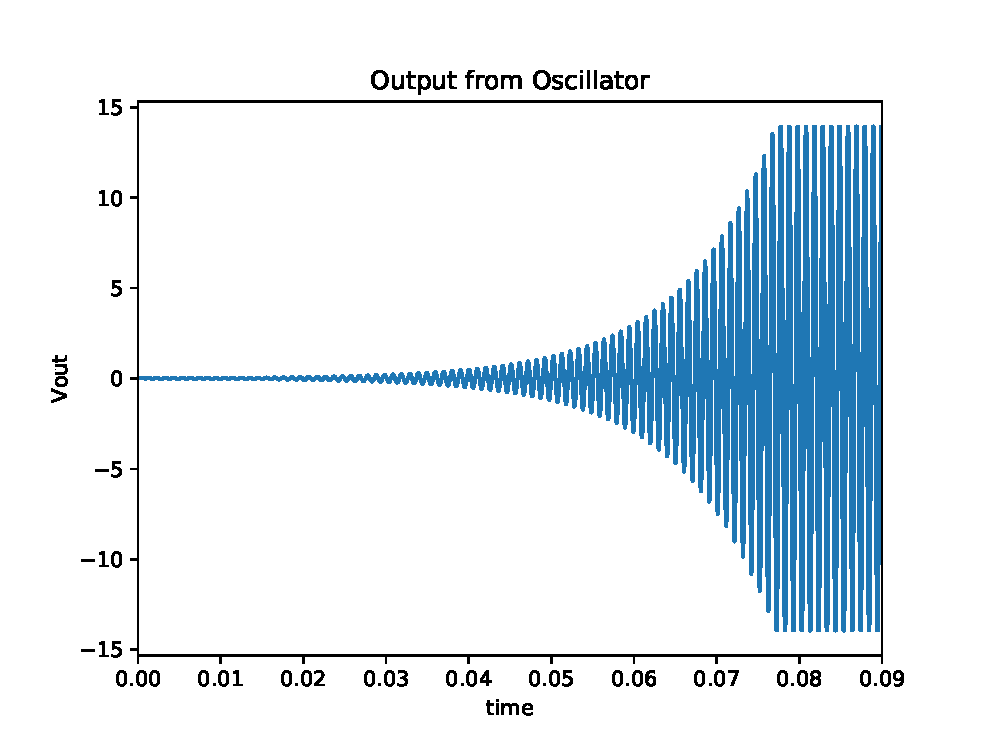
\includegraphics[width=\columnwidth]{./figs/ee18btech11044_3_2.eps}
\caption{}
\end{figure}

\item Tabulate the values of Resistors and Capacitors you have chosen for the simulation.

\solution

\begin{table}[!ht]
\centering
%%%%%%%%%%%%%%%%%%%%%%%%%%%%%%%%%%%%%%%%%%%%%%%%%%%%%%%%%%%%%%%%%%%%%%
%%                                                                  %%
%%  This is the header of a LaTeX2e file exported from Gnumeric.    %%
%%                                                                  %%
%%  This file can be compiled as it stands or included in another   %%
%%  LaTeX document. The table is based on the longtable package so  %%
%%  the longtable options (headers, footers...) can be set in the   %%
%%  preamble section below (see PRAMBLE).                           %%
%%                                                                  %%
%%  To include the file in another, the following two lines must be %%
%%  in the including file:                                          %%
%%        \def\inputGnumericTable{}                                 %%
%%  at the beginning of the file and:                               %%
%%        \input{name-of-this-file.tex}                             %%
%%  where the table is to be placed. Note also that the including   %%
%%  file must use the following packages for the table to be        %%
%%  rendered correctly:                                             %%
%%    \usepackage[latin1]{inputenc}                                 %%
%%    \usepackage{color}                                            %%
%%    \usepackage{array}                                            %%
%%    \usepackage{longtable}                                        %%
%%    \usepackage{calc}                                             %%
%%    \usepackage{multirow}                                         %%
%%    \usepackage{hhline}                                           %%
%%    \usepackage{ifthen}                                           %%
%%  optionally (for landscape tables embedded in another document): %%
%%    \usepackage{lscape}                                           %%
%%                                                                  %%
%%%%%%%%%%%%%%%%%%%%%%%%%%%%%%%%%%%%%%%%%%%%%%%%%%%%%%%%%%%%%%%%%%%%%%



%%  This section checks if we are begin input into another file or  %%
%%  the file will be compiled alone. First use a macro taken from   %%
%%  the TeXbook ex 7.7 (suggestion of Han-Wen Nienhuys).            %%
\def\ifundefined#1{\expandafter\ifx\csname#1\endcsname\relax}


%%  Check for the \def token for inputed files. If it is not        %%
%%  defined, the file will be processed as a standalone and the     %%
%%  preamble will be used.                                          %%
\ifundefined{inputGnumericTable}

%%  We must be able to close or not the document at the end.        %%
	\def\gnumericTableEnd{\end{document}}


%%%%%%%%%%%%%%%%%%%%%%%%%%%%%%%%%%%%%%%%%%%%%%%%%%%%%%%%%%%%%%%%%%%%%%
%%                                                                  %%
%%  This is the PREAMBLE. Change these values to get the right      %%
%%  paper size and other niceties.                                  %%
%%                                                                  %%
%%%%%%%%%%%%%%%%%%%%%%%%%%%%%%%%%%%%%%%%%%%%%%%%%%%%%%%%%%%%%%%%%%%%%%

	\documentclass[12pt%
			  %,landscape%
                    ]{report}
       \usepackage[latin1]{inputenc}
       \usepackage{fullpage}
       \usepackage{color}
       \usepackage{array}
       \usepackage{longtable}
       \usepackage{calc}
       \usepackage{multirow}
       \usepackage{hhline}
       \usepackage{ifthen}

	\begin{document}


%%  End of the preamble for the standalone. The next section is for %%
%%  documents which are included into other LaTeX2e files.          %%
\else

%%  We are not a stand alone document. For a regular table, we will %%
%%  have no preamble and only define the closing to mean nothing.   %%
    \def\gnumericTableEnd{}

%%  If we want landscape mode in an embedded document, comment out  %%
%%  the line above and uncomment the two below. The table will      %%
%%  begin on a new page and run in landscape mode.                  %%
%       \def\gnumericTableEnd{\end{landscape}}
%       \begin{landscape}


%%  End of the else clause for this file being \input.              %%
\fi

%%%%%%%%%%%%%%%%%%%%%%%%%%%%%%%%%%%%%%%%%%%%%%%%%%%%%%%%%%%%%%%%%%%%%%
%%                                                                  %%
%%  The rest is the gnumeric table, except for the closing          %%
%%  statement. Changes below will alter the table's appearance.     %%
%%                                                                  %%
%%%%%%%%%%%%%%%%%%%%%%%%%%%%%%%%%%%%%%%%%%%%%%%%%%%%%%%%%%%%%%%%%%%%%%

\providecommand{\gnumericmathit}[1]{#1} 
%%  Uncomment the next line if you would like your numbers to be in %%
%%  italics if they are italizised in the gnumeric table.           %%
%\renewcommand{\gnumericmathit}[1]{\mathit{#1}}
\providecommand{\gnumericPB}[1]%
{\let\gnumericTemp=\\#1\let\\=\gnumericTemp\hspace{0pt}}
 \ifundefined{gnumericTableWidthDefined}
        \newlength{\gnumericTableWidth}
        \newlength{\gnumericTableWidthComplete}
        \newlength{\gnumericMultiRowLength}
        \global\def\gnumericTableWidthDefined{}
 \fi
%% The following setting protects this code from babel shorthands.  %%
 \ifthenelse{\isundefined{\languageshorthands}}{}{\languageshorthands{english}}
%%  The default table format retains the relative column widths of  %%
%%  gnumeric. They can easily be changed to c, r or l. In that case %%
%%  you may want to comment out the next line and uncomment the one %%
%%  thereafter                                                      %%
\providecommand\gnumbox{\makebox[0pt]}
%%\providecommand\gnumbox[1][]{\makebox}

%% to adjust positions in multirow situations                       %%
\setlength{\bigstrutjot}{\jot}
\setlength{\extrarowheight}{\doublerulesep}

%%  The \setlongtables command keeps column widths the same across  %%
%%  pages. Simply comment out next line for varying column widths.  %%
\setlongtables

\setlength\gnumericTableWidth{%
	53pt+%
	93pt+%
0pt}
\def\gumericNumCols{2}
\setlength\gnumericTableWidthComplete{\gnumericTableWidth+%
         \tabcolsep*\gumericNumCols*2+\arrayrulewidth*\gumericNumCols}
\ifthenelse{\lengthtest{\gnumericTableWidthComplete > \linewidth}}%
         {\def\gnumericScale{\ratio{\linewidth-%
                        \tabcolsep*\gumericNumCols*2-%
                        \arrayrulewidth*\gumericNumCols}%
{\gnumericTableWidth}}}%
{\def\gnumericScale{1}}

%%%%%%%%%%%%%%%%%%%%%%%%%%%%%%%%%%%%%%%%%%%%%%%%%%%%%%%%%%%%%%%%%%%%%%
%%                                                                  %%
%% The following are the widths of the various columns. We are      %%
%% defining them here because then they are easier to change.       %%
%% Depending on the cell formats we may use them more than once.    %%
%%                                                                  %%
%%%%%%%%%%%%%%%%%%%%%%%%%%%%%%%%%%%%%%%%%%%%%%%%%%%%%%%%%%%%%%%%%%%%%%

\ifthenelse{\isundefined{\gnumericColA}}{\newlength{\gnumericColA}}{}\settowidth{\gnumericColA}{\begin{tabular}{@{}p{53pt*\gnumericScale}@{}}x\end{tabular}}
\ifthenelse{\isundefined{\gnumericColB}}{\newlength{\gnumericColB}}{}\settowidth{\gnumericColB}{\begin{tabular}{@{}p{93pt*\gnumericScale}@{}}x\end{tabular}}

\begin{tabular}[c]{%
	b{\gnumericColA}%
	b{\gnumericColB}%
	}

%%%%%%%%%%%%%%%%%%%%%%%%%%%%%%%%%%%%%%%%%%%%%%%%%%%%%%%%%%%%%%%%%%%%%%
%%  The longtable options. (Caption, headers... see Goosens, p.124) %%
%	\caption{The Table Caption.}             \\	%
% \hline	% Across the top of the table.
%%  The rest of these options are table rows which are placed on    %%
%%  the first, last or every page. Use \multicolumn if you want.    %%

%%  Header for the first page.                                      %%
%	\multicolumn{2}{c}{The First Header} \\ \hline 
%	\multicolumn{1}{c}{colTag}	%Column 1
%	&\multicolumn{1}{c}{colTag}	\\ \hline %Last column
%	\endfirsthead

%%  The running header definition.                                  %%
%	\hline
%	\multicolumn{2}{l}{\ldots\small\slshape continued} \\ \hline
%	\multicolumn{1}{c}{colTag}	%Column 1
%	&\multicolumn{1}{c}{colTag}	\\ \hline %Last column
%	\endhead

%%  The running footer definition.                                  %%
%	\hline
%	\multicolumn{2}{r}{\small\slshape continued\ldots} \\
%	\endfoot

%%  The ending footer definition.                                   %%
%	\multicolumn{2}{c}{That's all folks} \\ \hline 
%	\endlastfoot
%%%%%%%%%%%%%%%%%%%%%%%%%%%%%%%%%%%%%%%%%%%%%%%%%%%%%%%%%%%%%%%%%%%%%%

\hhline{|-|-}
	 \multicolumn{1}{|p{\gnumericColA}|}%
	{\gnumericPB{\centering}\gnumbox{\textbf{Parameter}}}
	&\multicolumn{1}{p{\gnumericColB}|}%
	{\gnumericPB{\centering}\gnumbox{\textbf{Value}}}
\\
\hhline{|--|}
	 \multicolumn{1}{|p{\gnumericColA}|}%
	{\gnumericPB{\raggedright}\gnumbox[l]{$R_{1}$}}
	&\multicolumn{1}{p{\gnumericColB}|}%
	{\gnumericPB{\raggedright}\gnumbox[l]{$10k\Omega$}}
\\
\hhline{|--|}
	 \multicolumn{1}{|p{\gnumericColA}|}%
	{\gnumericPB{\raggedright}\gnumbox[l]{$R_{2}$}}
	&\multicolumn{1}{p{\gnumericColB}|}%
	{\gnumericPB{\raggedright}\gnumbox[l]{$20.3k\Omega$}}
\\
\hhline{|--|}
	 \multicolumn{1}{|p{\gnumericColA}|}%
	{\gnumericPB{\raggedright}\gnumbox[l]{$R_{p}$}}
	&\multicolumn{1}{p{\gnumericColB}|}%
	{\gnumericPB{\raggedright}\gnumbox[l]{$10k\Omega$}}
\\
\hhline{|--|}
	 \multicolumn{1}{|p{\gnumericColA}|}%
	{\gnumericPB{\raggedright}\gnumbox[l]{$R_{s}$}}
	&\multicolumn{1}{p{\gnumericColB}|}%
	{\gnumericPB{\raggedright}\gnumbox[l]{$10k\Omega$}}
\\
\hhline{|--|}
	 \multicolumn{1}{|p{\gnumericColA}|}%
	{\gnumericPB{\raggedright}\gnumbox[l]{$C_{s}$}}
	&\multicolumn{1}{p{\gnumericColB}|}%
	{\gnumericPB{\raggedright}\gnumbox[l]{$16nF$}}
\\
\hhline{|--|}
	 \multicolumn{1}{|p{\gnumericColA}|}%
	{\gnumericPB{\raggedright}\gnumbox[l]{$R_{p}$}}
	&\multicolumn{1}{p{\gnumericColB}|}%
	{\gnumericPB{\raggedright}\gnumbox[l]{$10k\Omega$}}
\\
\hhline{|--|}
	 \multicolumn{1}{|p{\gnumericColA}|}%
	{\gnumericPB{\raggedright}\gnumbox[l]{$C_{p}$}}
	&\multicolumn{1}{p{\gnumericColB}|}%
	{\gnumericPB{\raggedright}\gnumbox[l]{$16nF$}}

\\
\hhline{|-|-|}
\end{tabular}

\ifthenelse{\isundefined{\languageshorthands}}{}{\languageshorthands{\languagename}}
\gnumericTableEnd

\caption{}
\label{table:ee18btech11044_t_1}
\end{table}

Where, according to Fig \ref{fig:ee18btech11044_3_tikz_1}
\begin{align}
    R_p = R_s = R \\
    C_p = C_s = C
\end{align}
 
 \item Calculate the frequency of sinusoidal generated for the combination of R and C chosen using Eq \ref{eq:ee18btech11044_3_4}
 
 \solution
 
 Frequency generated is given by 
 
 \begin{align}
     \omega_{0} = \frac{1}{ R C} \\
     \omega_{0} = 6250 rad/sec \\
     f_{0} = 995.22Hz.
 \end{align}
 
 \item Calculate the frequency of sinusoidal wave using plot generated from simulation.
 
 \solution
 \begin{itemize}
     \item Consider a part of plot generated from simulation shown in the Fig \ref{fig:ee18btech11044_3_plot_3}.
     \item Calculating the Time-period of the sinusoidal wave generated using the two points marked in the Fig \ref{fig:ee18btech11044_3_plot_3}.
     \begin{align}
         T_0 = 0.0856452 - 0.0846361 \\
         f_0 = 1/T_0 \\
         f_0 = 990.98Hz.
     \end{align}
     \item We get the frequencies calculated from the formulae and the plot to be approximately same.
 \end{itemize}
 
 
 \begin{figure}[!ht]
\centering
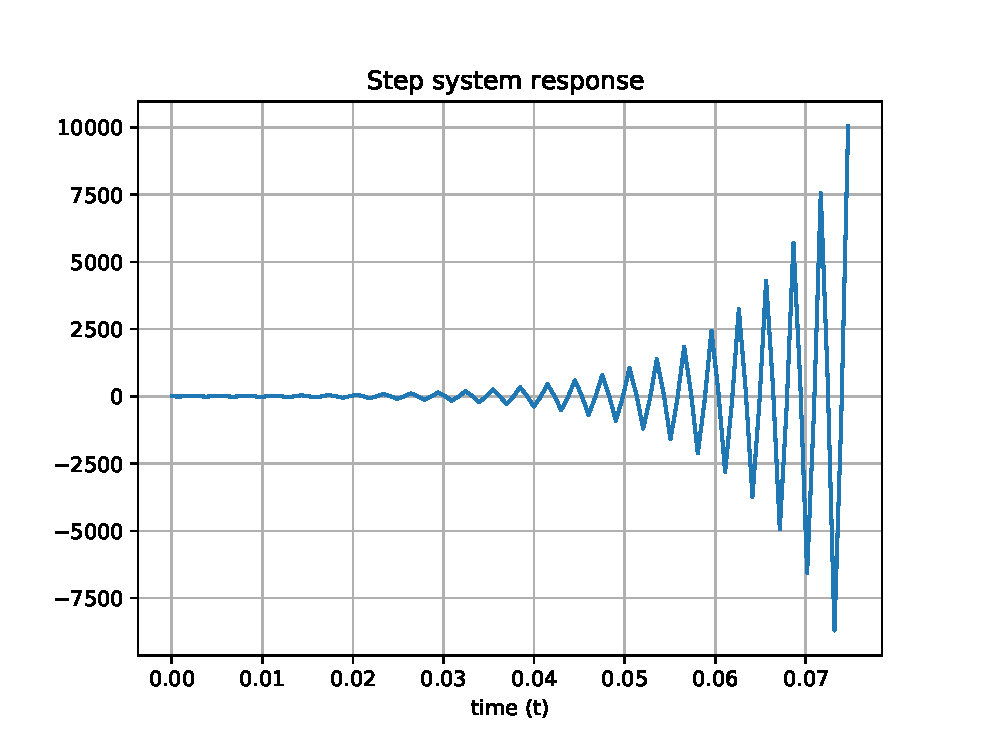
\includegraphics[width=\columnwidth]{./figs/ee18btech11044_3_3.eps}
\caption{}
\label{fig:ee18btech11044_3_plot_3}
\end{figure}
\end{enumerate}
